%\graphicspath{{D:/project/thesis_preparation/PhDtemplateLATEX_V2/ch_Background_Work/figures/}}
\section{Magnetic Resonance Imaging}
Magnetic Resonance Imaging (MRI) is an imaging technology that allows non-invasive visualization of the body using magnetic fields. It is a crucial enabler of modern healthcare and medical research and is used for the detection and diagnosis of neuropathology.

MRI is based on the principles of nuclear magnetic resonance (NMR), where atomic nuclei, when placed in a magnetic field, can absorb and emit electromagnetic radiation. An MRI machine applies a primary magnetic field (B0) to magnetize and align the hydrogen nuclei in the body. A radio frequency (RF) field is subsequently introduced perpendicular to B0, and reorients the spin axis. This causes the nuclei to produce NMR signals detectable by the MRI scanner. Based on the precession frequency decay, the signals are recorded to construct an image of the scanned area based on the contrasts in water and fat concentrations \cite{Plewes2012,Johansen-Berg2013}. 

\subsection{Basic Principles}
\subsubsection{Spin and Magnetic Moment}
Spin is an intrinsic property of elementary particles, and can be either positive or negative. The spin quantum number  $s$ is defined as $ s = \frac{n}{2}$, where $n \in \{0,1,2,...\}$. Therefore $s$ is a quantized value in multiples of $\frac{1}{2}$. Protons, electrons and neutrons possess spin. Nuclei with an odd number of protons or neutrons have non-zero nuclear spins; while those with an even number of protons and neutrons have no spin. Particles with opposite spins can pair up to produce an overall spin of zero. Hydrogen nuclei, which makes up 63$\%$ the human body, possess spins of $\frac{1}{2}$. The spin of a particle has a magnetic moment vector that behaves like a magnet with north and south poles (Figure \ref{fig:spin}).


\begin{figure}[h]
\begin{center}
\begin{tabular}{c}
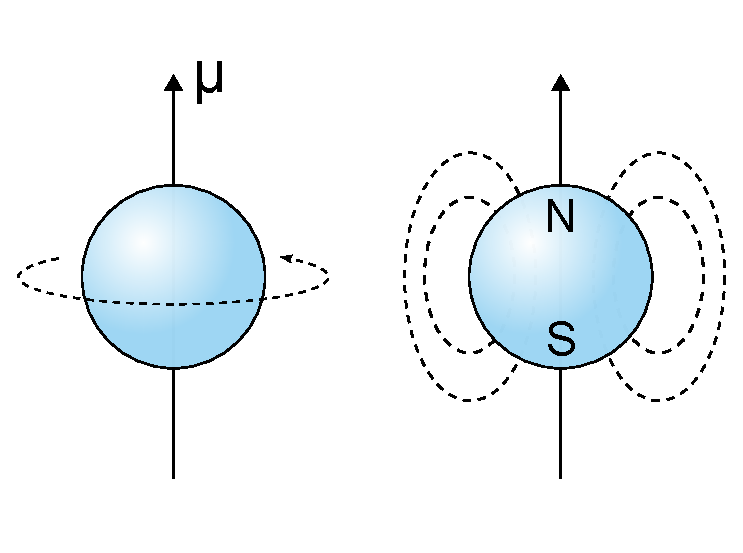
\includegraphics[width=3.5in]{mri/spin.pdf}
\end{tabular}
\caption{Spin of a nucleus has a magnetic moment vector $\mu$, which behaves similar to a magnet with north (N) and south (S) poles.}
\label{fig:spin}
\end{center}
\end{figure}

The spinning of nuclear particles produces angular momentum  $\textbf{J}$, that is a vector with both magnitude and direction. The largest measurable component of $J$, expressed as $I$, represents the overall quantized spin value as the spin quantum number. The corresponding quantum number is known as the magnetic quantum number $m$, and can take a total of $2I + 1$ angular momentum states.  A non-zero spin is associated with a non-zero magnetic moment ($\vec{\mu}$) via the relation $\vec{\mu} =\gamma \textbf{J}$. The z-component of the angular momentum vector (\textbf{J}) is $J_z = m \hbar$. The z-component of the magnetic moment $\mu_z$ is thus: 

$$\mu_z=\gamma J_z=\gamma m \hbar$$

Where $\gamma$ is the gyromagnetic ratio, $\hbar$ is the reduced Planck constant ($=1.0545726 \times 10^{-34} m^2kg/s$ ).

\subsubsection{Effect of Magnetic Field}

In the absence of an externally applied magnetic field, the magnetic dipoles are oriented randomly. When the proton is placed in an external magnetic field $B_0$, the spin vectors become oriented with the field, either parallel or anti-parallel with respect to $B_0$ (Figure \ref{fig:externalB0}). The nuclei precess about the magnetic field direction at some frequency called Larmor frequency: 

$$\omega = \gamma B$$.

Where $\gamma$ is the gyromagnetic ratio, and $B$ the magnetic field magnitude.


\begin{figure}[h]
\begin{center}
\begin{tabular}{c}
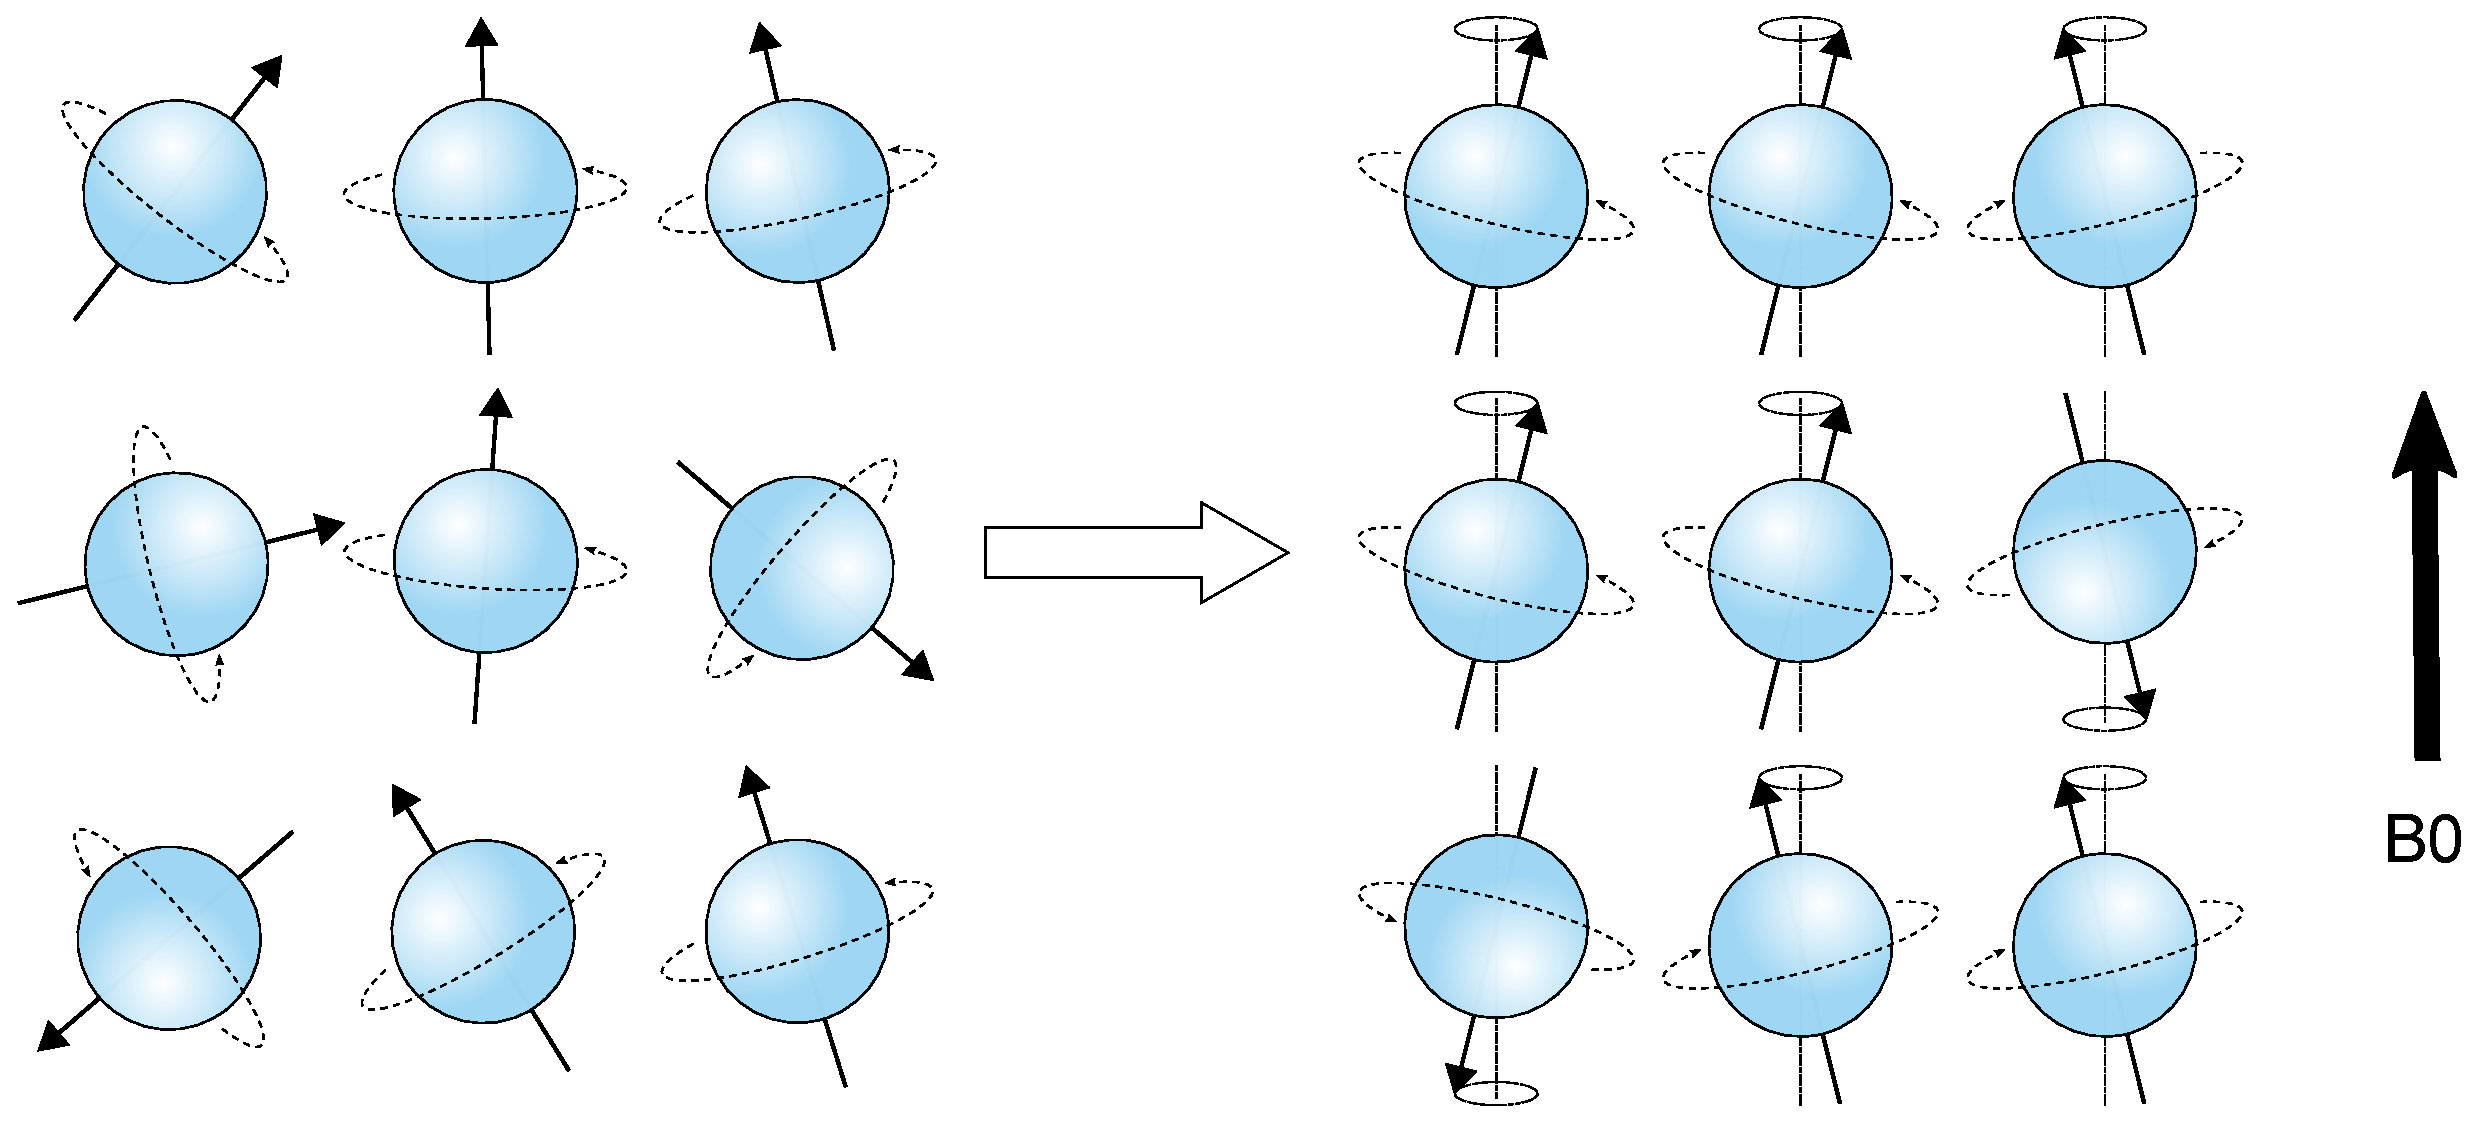
\includegraphics[width=4.5in]{mri/field.pdf}
\end{tabular}
\caption{Left panel-- magnetic moments with random orientations in the absence of external magnetic field; Right panel-- magnetic moments parallel or anti-parallel aligned with the external
field} \label{fig:externalB0}
\end{center}
\end{figure}

Protons aligned in the parallel alignment are more preferred as they have a lower energy state than protons in anti-parallel orientation. The energy E of a magnetic moment $\vec{\mu}$ when in a magnetic field $B_0$ is given by: $E=-\vec{\mu}\cdot \textbf{B}_0=-\mu_z B_0=-\gamma m \hbar B_0$. The lower energy state of protons corresponding to m = +1/2 in a static magnetic field $B_0$ is $E(\frac{1}{2})=-\frac{1}{2}\gamma \hbar B_0$. The higher energy state of protons corresponding to m =-1/2 is given by $E(-\frac{1}{2})=\frac{1}{2}\gamma \hbar B_0$.
Consequently, the energy differences between two quantum states can be calculated as $\bigtriangleup E = \gamma \hbar B_0$ (Figure \ref{fig:energy}).

\begin{figure}[h]
\begin{center}
\begin{tabular}{c}
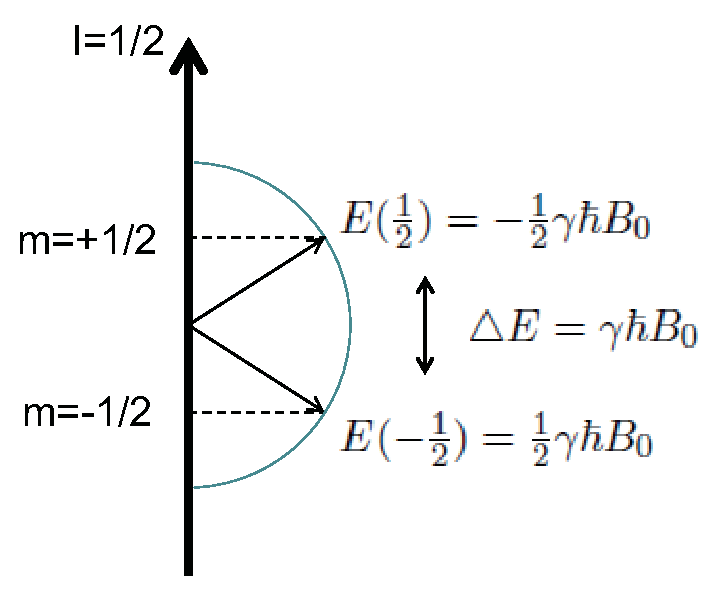
\includegraphics[width=3in]{mri/energy}
\end{tabular}
\caption{For protons with spin quantum number of 1/2, two energy
levels and the energy difference are shown.} \label{fig:energy}
\end{center}
\end{figure}

There are more protons with spins with parallel orientation than anti-parallel, due to the increased energy stability. This number of difference is called spin excess and the magnetic moments of the excess spins add to form the net magnetization vector $M_z$. When the spin system is at equilibrium, net magnetization lies along the z-axis, parallel to $B_0$.

\subsubsection{Resonance Condition}

The steady-state of the stable spin state under $B_0 $ can be disturbed by introducing additional energy $E$ into the system. 

The proton would undergo a transition from the lower energy to higher energy state by the absorption of a photon. The energy difference between the nuclear spin levels is $\bigtriangleup E = \gamma \hbar B_0$. Hence, a magnetic resonance absorption will only occur when $\nu_0 = \gamma B_0/(2 \pi)$, which is the same as Larmor frequency. This is called the \textit{resonance condition}. 

\subsubsection{Relaxation}
Transverse magnetization is introduced into the system that oscillates at radio frequency (RF) to modify the net magnetization, and this is called the RF pulse. When exposing the nuclear spin system to the energy of the RF pulse, the equilibrium of the spin system is disturbed. The RF pulse is designed to introduce energy E such that the net spin direction orients at $90^\circ$. The net magnetization now is denoted as $M_{xy}$ as it aligns with the xy-plane instead of the z-axis. Individual spins now precess in phase with the RF pulse, and it gives rises to the MR signal in the receiver coil. 

With the termination of the RF pulse, the nuclei in the excited state will return to the equilibrium condition. This process is called \textit{relaxation}. 
The energy transmitted decays rapidly by two relaxation processes:  spin-lattice and spin-spin relaxations. These are responsible for \textit{T1 relaxation} and \textit{T2 relaxation} respectively.

\paragraph{T1 Relaxation} 
As the transverse magnetization decays, the magnetic moment gradually realigns with the z-axis of $B_0$. 
The magnitude of the magnetic moment's xy-component also gradually diminishes, and the MR signal fades. 
The $M_z$ magnetic moment recovers in proportion, and is eventually restored. 
This processed is called \textit{longitudinal relaxation} or T1 recovery, where T1 refers to the mean time for an individual nucleus to
dissipate its excess energy (heat) to the surrounding environment ( the \textit{lattice}, and therefore the processed is also named \textit{spin-lattice relaxation})and return to its equilibrium state. 

\begin{figure}[htb]
\begin{center}
\begin{tabular}{c}
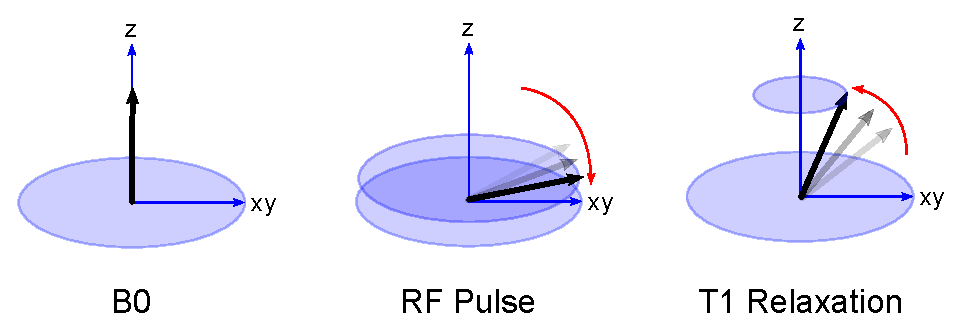
\includegraphics[width=\textwidth]{mri/rf-pulse.pdf}
\end{tabular}
\caption{Illustration of the process of transverse relaxation. Initially, the net magnetization orientes to the B0 field under steady-state. When a 90 deg RF pulse is applied, the spin orients towards the xy-plane. When the RF pulse is switched off, the spin now relaxes towards the z-axis.  } \label{fig:relaxation}
\end{center}
\end{figure}

To describe how $M_z$ returns from 0 to its equilibrium during relaxation, the equation as a
function with respect to time $t$ is written as: 
$$M_z = M_0 (1 - e^{-t/T1})$$
where T1 is the time taken for approximately 63$\%$ of the longitudinal magnetization to be restored (Figure \ref{fig:T1T2}(A)). 
$M_0$ is the magnetic moment at equilibrium. 

\paragraph{T2 Relaxation}

T2 relaxation is so named after the time constant of phase decoherence of the transverse magnetic moment. 

Immediate after excitation, the phase precessions are synchronous, and therefore are in \textit{phase coherence}.  
However due to the following reasons, the various spins begin to lose coherence, and their total sum magnetization $M_xy$ diminishes. 

Phase coherence is lost in two ways:
\begin{enumerate}
\item Spins are associated with local magnetic fields, and interact randomly. The energy transfers that occur in the local magnetic field interactions cause a cumulative loss of phase. These are pure spin-spin interactions, and thereby not affected by $180^\circ$ refocusing pulse. They are also independent of the strength of $B_0$. 
The time constant which describes the return to equilibrium of the transverse magnetization is called the \textit{spin-spin
relaxation time} or T2, and is defined in respect to time $t$ as:
$$M_{xy} =M_{xymax} e^{-t/T2}$$
where T2 is the duration of time for the transverse magnetization to decay to 37$\%$ of its original magnitude. 
T2 is always less than or equal to T1.

\item There are intrinsic inhomogeneities by the main static magnetic field generator, and the scanning subject. These intrinsic properties contribute to the dephasing, and has a shorter time decay than T2. This type of decay time constant is named T2*  (Figure \ref{fig:T1T2}(C)). The loss of the MR signal due to T2* is called\textit{ free induction decay} (FID). T2* is defined as follows: 
$$ \frac{1}{T_2^*} = \frac{1}{T_2} + \frac{1}{T_2inhomo}$$ 
\end{enumerate}

\begin{figure}[ht]
\begin{center}
\begin{tabular}{c}
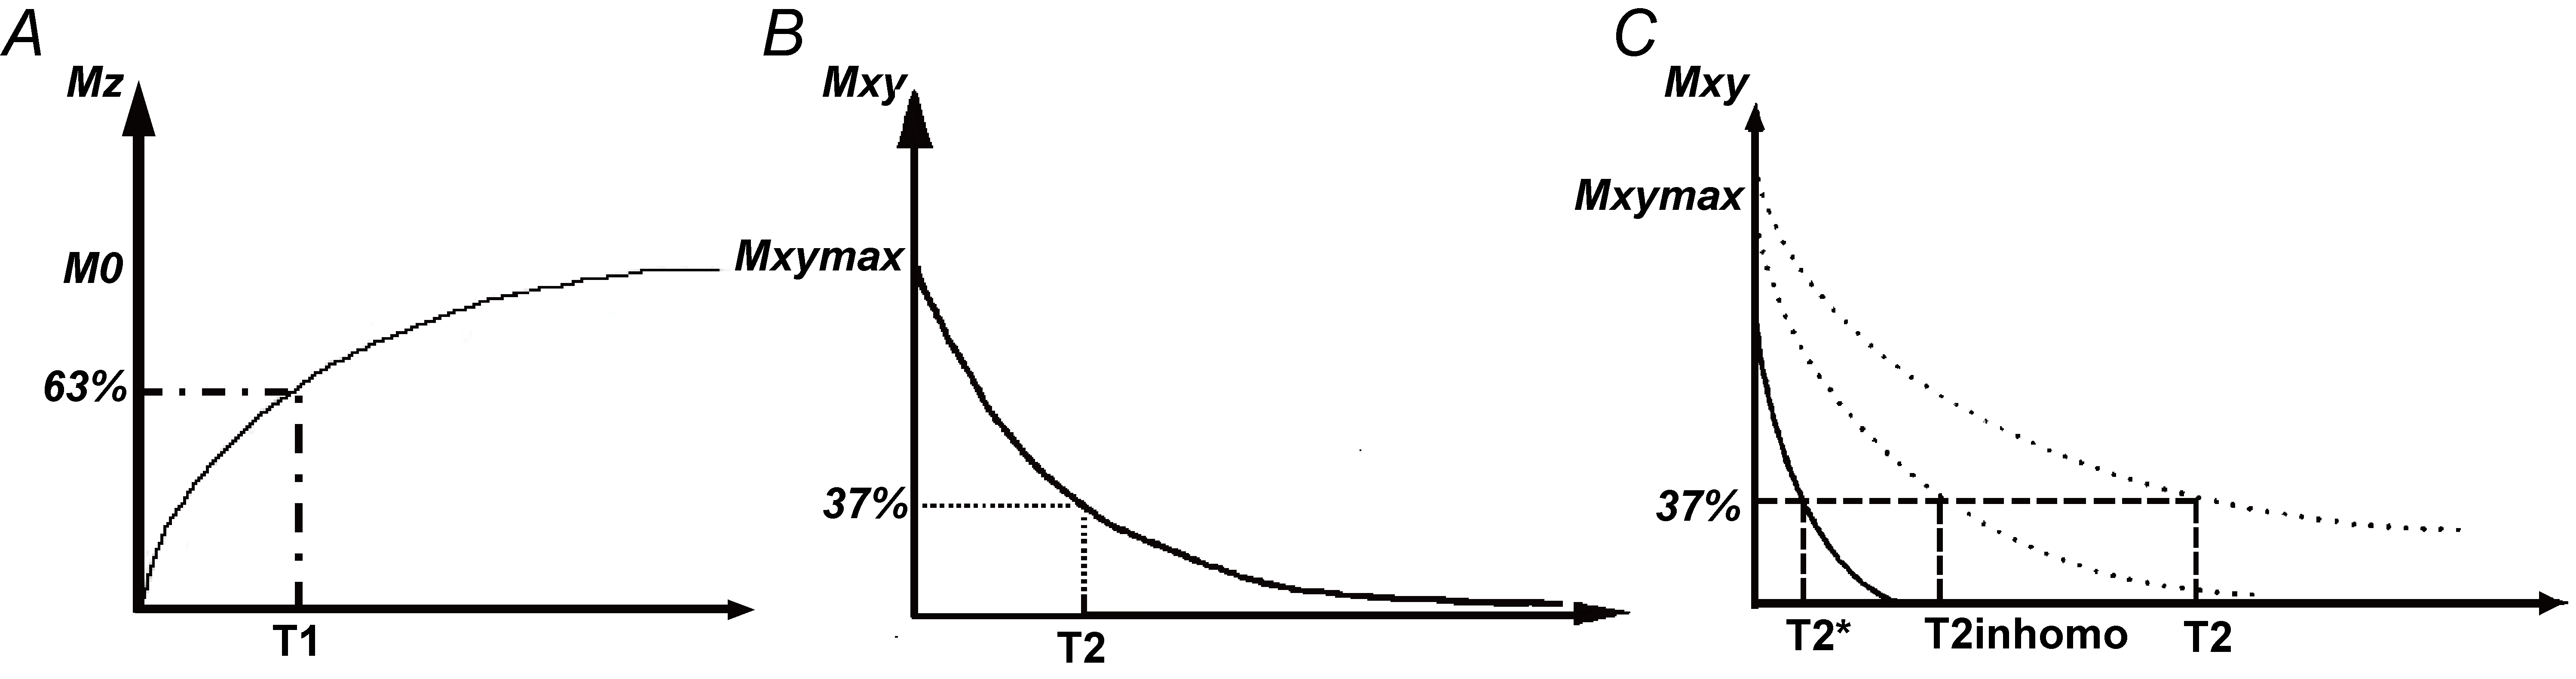
\includegraphics[width=5.5in]{mri/T1T2}
\end{tabular}
\caption{Diagram depicting the relaxation processes of T1 (panel A), T2 (panel B) and $T_2^*$ (panel C). $T_2^*$ is shorter than T2.} \label{fig:T1T2}
\end{center}
\end{figure}

\subsubsection{MR Contrast}

MRI signal intensity depends primarily on three parameters: 
\begin{itemize}
\item Proton density: the number of excitable spins per unit volume, which determines the maximum amount of signal that can be measured from the tissue. It can be measured by minimizing T1 and maximizing T2 times. 
\item T1 time: the amount time for $M_xy$ to recover to $M_z$, to be ready for re-excitation.
\item T2 time: the amount of time for $M_xy$ signal to fade under decoherence. 
\end{itemize}
The contrast in brain tissues of the resulting MR image can be tuned by adjusting T1  and T2 parameters in pulse sequence design.

\paragraph{Repetition Time}
T1 contrast is adjusted by tuning repetition time (TR), which is the length of relaxation interval between excitation pulses. When TR is long (\textgreater 1500 ms), $M_z$ recovers totally, and therefore subsequent excitation will again retain maximal signal strength. When the TR is short (
\textless 600 ms), the $M_z$ has not entirely recovered, and the next excitation pulse will not be able to regain signal strength. Different tissues have different intrinsic T1 differences, and will show strong contrast under short TR. Therefore short TR are said to be T1 weighted. 

\paragraph{Echo Time}
MR sequences have a gradient field which is used to encode spatial origin. The gradients also contribute to spin dephasing. In spin echo imaging, a 90 deg pulse and a 180 deg refocusing pulse are needed to measure MR signals adequately. The time delay between the first pulse and the measured signal under phase coherence (spin echo) is known as echo time (TE). When TE is short ($<$ 30 ms), and TR is short, the image is said to be T1 weighted; when TE is long ( $\geq$ 60 ms ), and TR is long, the image is said to be T2-weighted. 

\begin{figure}[htb]
\begin{center}
\begin{tabular}{c}
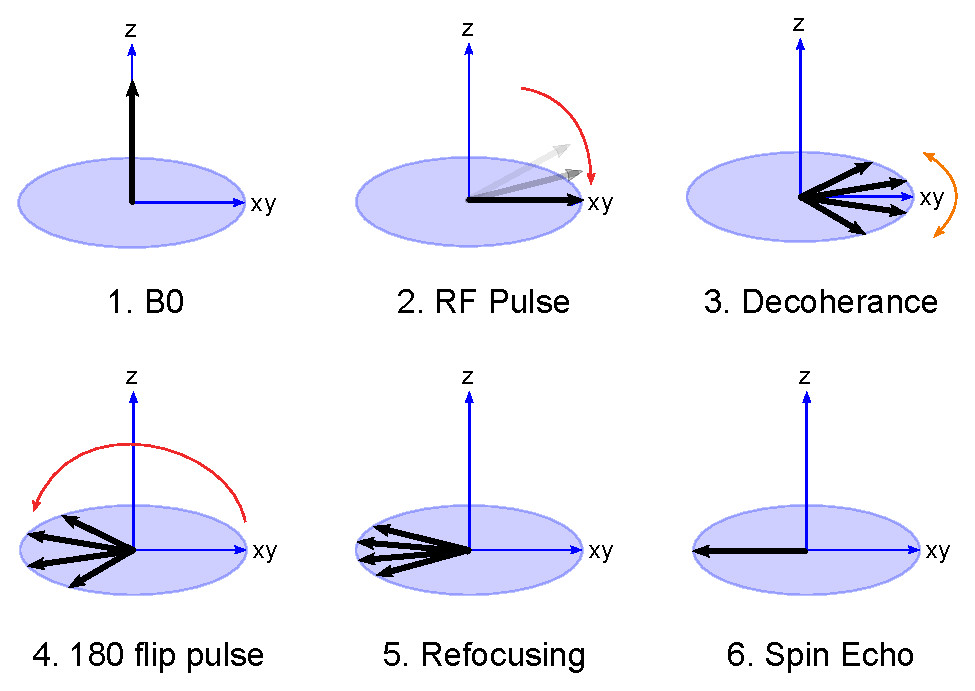
\includegraphics[width=\textwidth]{mri/spin-echo-2.pdf}
\end{tabular}
\caption{Illustration of the process of spin-echo. Initially, the spins orients to wards B0 field under steady-state. When a 90deg RF pulse is applied, the spins orients to the xy-plane. When the RF pulse is switched off, the spins undergoe phase decoherence. A 180 degrees refocusing pulse is applied to bring spins back into coherence, at which point in time the peak of an "echo" occurs.  } \label{fig:spin-echo}
\end{center}
\end{figure}

Typically, T1-weighted spin echo (SE)  sequence is acquired with TR \textless 800 ms, TE \textless 20 ms; T2-weighted fast spin echo (FSE) at TR \textgreater 2000 ms, TE \textgreater 60 ms. 
In the case of T1-weighted MRI, images are created with short TE and short TR times. They can differentiate fat from water - with fat brighter and water darker (\url{www.mr-tip.com}) by using a gradient echo (GRE) sequence. In the brain T1-weighted scans provide good gray matter/white matter contrast. In addition, the image contrast can be increased with the use of an inversion pulse as in an MP-RAGE sequence. Due to short TR, this scan can be run very quickly, allowing the collection of high resolution 3D structural image (Figure \ref{fig:T1T2PD}, Left). These structural images can provide detailed information on the brain's shape and size, and provide the base for cortical surface reconstruction and segmentation. 

The T2-weighted sequence uses a long TR and long TE. The T2-weighted sequence can be employed as a multi-echo sequence. Like the T1-weighted scan, fat is
differentiated from water in single echo sequences, but with fat dark and water bright (Figure \ref{fig:T1T2PD}, Middle).  

Another type of image with shorter echo ($T_E<30msec$) is proton density (PD) (Figure \ref{fig:T1T2PD}, right) weighted. This image provides poor contrast of tissue and CSF, but good bright contrast against lesions, thus very helpful for evaluating periventricular pathology . $T_2^*$-weighted scans use a gradient echo (GRE) sequence, which uses only one RF pulse and gradient reversal. It is prone to susceptibility losses at air/tissue boundaries, but can increase contrast for certain types of tissue, such as venous blood. It is used for functional MRI detection allowing people to visualize and map the parts of the brain used to perform tasks. 

\subsubsection{3D encoding}

\paragraph{Slice Selection} Recall that the resonance condition can only be satisfied when the RF pulse is equal to the Larmor frequency of the nucleus precession under the magnetic field. 
Therefore, to allow slice discrimination, the magnetic field along the z-axis is made to be inhomogeneous by introducing a linear gradient field. It is an extra coil that adds or subtracts from the main magnetic field. With the linear gradient, only a particular portion of the z-axis would share a similar unique Larmor frequency, and can be selectively excited with an RF pulse. The steepness of the gradient determines the slice thickness, the steeper the gradient, the thinner the slices.  

\paragraph{Spatial Encoding}
Once the spins are excited and precess in the xy-plane, two additional gradients are applied to allow discrimination of signal measures per slice. 

\begin{itemize}
\item Phase encoding: The phase encoding gradient is applied in the y-direction. It temporarily alters the Larmor frequency of the spins based their location of the y-axis, and results in phase shifts of the spins relative to each other. The phase shift is determined by the duration and amplitude of the gradient, when the gradient is switched off, all spins return to their initial rate of precession, but maintains the relative phase shift. 
\item Frequency encoding: The frequency encoding gradient is applied on the x-direction. This applies a magnetic field that increases in strength from right to left. The change in Larmor frequency alters the precession speed of the spins such that the spins towards the right precess faster than that of the left. The MR signal collected represents the entire frequency spectrum of the spins. 
\end{itemize}

The measured MR signal with both encoding methods allows recovery of spatial information from the scanned area. Application of Fourier transform will decompose the signal into component frequencies along the frequency encoding direction (x). The phase distribution along each frequency provide information on the phase encoding direction (y). Decomposing the phase distribution requires another Fourier transform on the multiple scans of different phase gradient strengths. This is called two-dimensional Fourier transform (2D-FT), the number of phase gradient measures is called the phase encoding step. 

\paragraph{K-Space}

The collected MR data are encoded in a mathematical space termed the k-space. The k-space is a two-dimensional feature space, where the x-axis $k_x$ represent the measured frequency domain, and $k_y$ the phase domain. Each step in $k_y$ represents a single phase encoding step. The x-axis origin $k_x=0$ is the gradient iso-center, where the gradient magnetic field equals to zero, and the frequency distribution is symmetric about the x-origin. The 2D-FT operation is applied to the k-space to transform the frequency domain information into an image. 

\begin{figure}[htb]
\begin{center}
%\begin{tabular}{c}
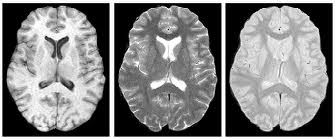
\includegraphics[width=5in]{mri/T1T2PD}
%\end{tabular}
\caption{Brain scan using T1 (left), T2 (middle) and proton density (right) measurements.}
\label{fig:T1T2PD}
\end{center}
%\vspace{-0.15in}

\end{figure}
